\section{Recognising optimality}

We now turn our focus to recognising whether a given point satisfy necessary and/or sufficient conditions for optimality. Even though these conditions can be used to test if a candidate point is optimal for a problem, its most important use is serving as a framework for directing solution methods in their search for optimal solutions. 

Before we proceed, let us define the terminology we will use to refer to solutions. Let $f:\reals^n \mapsto \reals$. Consider the problem
$(P) :~ \mini\braces{f(x) : x \in S}$.
% 
\begin{enumerate}
\item a \emph{feasible solution} is any solution  $\overline{x} \in S$;
\item a \emph{local optimal solution} is a feasible solution $\overline{x}\in S$ that has a neighbourhood $N_\epsilon(\overline{x}) = \braces{x : ||x - \overline{x}|| \leq \epsilon}$ for some $\epsilon >0$ such that $f(\overline{x}) \leq f(x)$ for each $x \in S \cap N_\epsilon(\overline{x})$.
\item a \emph{global optimal solution} is a feasible solution $\overline{x} \in S$ with $f(\overline{x}) \leq f(x)$ for all $x \in S$. Or alternatively, is a local optimal solution for which $S \subseteq N_\epsilon(\overline{x})$.
\end{enumerate}
%
Figure \ref{fig:example_optima} illustrates the concepts above. Solution $x_1$ is an unconstrained global minimum, but is not a feasible solution considering the feasibility set $S$. Solution $x_2$ is a local optima, for any neighbourhood $N_\epsilon(x_2)$ only encompassing the points within the same plateau. Solution $x_3$ is a local optimum, while $x_4$ is neither a local or a global optimum in the unconstrained case, but is a global maximum in the constrained case. Finally, $x_5$ is the global minimum in the constrained case.

\begin{figure}
	\begin{subfigure}{\textwidth}
	\centering
		\begin{tikzpicture}
	%			\draw[help lines] (-5,-3) grid (5,3);
			\node (pic) at (0,0) {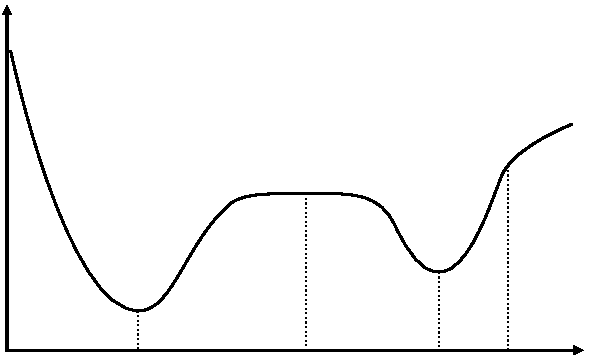
\includegraphics{part_2/chapter_4/figures/unconstrained.pdf}};
			\node (f) at (-4.3, 3.1) {$f(x)$};
			\node (x) at (5.1, -3) {$x$};
			\node (x1) at (-2.65,-3.2) {$x_1$};
			\node (x2) at (0.2,-3.2) {$x_2$};
			\node (x3) at (2.45,-3.2) {$x_3$}; 
			\node (x4) at (3.6,-3.2) {$x_4$}; 
		\end{tikzpicture}
		\caption{Unconstrained optimisation problem}\label{fig:unconstrained}	
	\end{subfigure}
	\begin{subfigure}{\textwidth}
	\centering
		\begin{tikzpicture}
%			\draw[help lines] (-5,-3) grid (5,3);
			\node (pic) at (0,0) {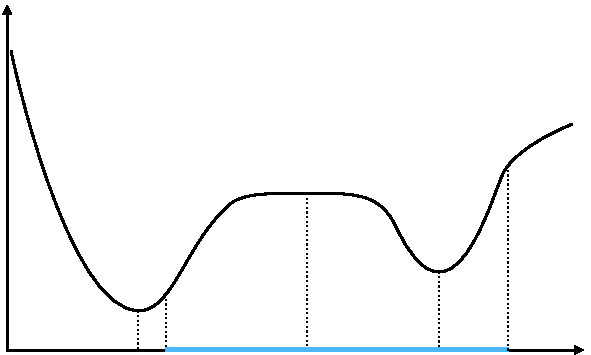
\includegraphics{part_2/chapter_4/figures/constrained.pdf}};
			\node (f) at (-4.3, 3.1) {$f(x)$};
			\node (x) at (5.1, -3) {$x$};
			\node (x1) at (-2.65,-3.2) {$x_1$};
			\node (x2) at (0.2,-3.2) {$x_2$};
			\node (x3) at (2.45,-3.2) {$x_3$}; 
			\node (x4) at (3.6,-3.2) {$x_4$};
			\node (x5) at (-2.1,-3.2) {$x_5$};
			\node (S) at (1.1,-2.5) {$S$}; 
		\end{tikzpicture}
		\caption{Constrained optimisation problem}\label{fig:constrained}		
	\end{subfigure}
	\caption{Points of interest in optimisation. Points $x_1$, $x_2$ and $x_3$ are local optima in the unconstrained problem. Once a constraint set $S$ is imposed, $x_4$ and $x_5$ become points of interest and $x_1$ becomes infeasible.} \label{fig:example_optima}		
\end{figure}


\section{The role of convexity in optimality conditions}


We can now state what is possibly the most important result in optimisation. In a nutshell, this results allows one promote local optimality to global optimality in the presence of convexity. 

\begin{theorem}[global optimality of convex problems]\label{thm:convex_global}
Let $S \subseteq \reals^n$ be a nonempty convex set and $f:S \mapsto \reals$ convex on $S$. Consider the problem $(P):~\mini \braces{f(x) : x \in S}$. Suppose $\overline{x}$ is a local optimal solution to $P$. Then $\overline{x}$ is a global optimal solution.
\end{theorem}

\begin{proof}
Since $\overline{x}$ is a local optimal solution, there exists $N_\epsilon(\overline{x})$ such that, for each $x \in S \cap N_\epsilon(\overline{x})$, $f(\overline{x}) \leq f(x)$. By contradiction, suppose $\overline{x}$ is not a global optimal solution. Then, there exists a solution $\hat{x} \in\hspace{-1pt} S$ so that $f(\hat{x}) < f(\overline{x})$. Now, for any $\lambda \in [0,1]$, the convexity of $f$ implies:  
%
\begin{align*}
f(\lambda\hat{x} + (1-\lambda)\overline{x}) \leq \lambda f(\hat{x}) + (1-\lambda)f(\overline{x}) < \lambda f(\overline{x}) + (1-\lambda)f(\overline{x}) = f(\overline{x})
\end{align*}
%
However, for $\lambda > 0$ sufficiently small, $\lambda\hat{x} + (1-\lambda)\overline{x} \in S\cap N_\epsilon(\overline{x})$ due to the convexity of $S$, which contradicts the local optimality of $\overline{x}$. Thus, $\overline{x}$ is a global optimum. 
\end{proof}

The proof is built using contradiction. That is, we show that for a solution to be a local optimum in a convex problem, not being a global solution contradicts its local optimality, originally true by assumption. This is achieved using the convexity of $f$ and showing that the convex combination between hypothetical better solution $\hat{x}$ and $\overline{x}$ would have to be both in $N_\epsilon(\overline{x})$ and better than $\overline{x}$, contradicting the local optimality of $\overline{x}$.


\section{Optimality condition of convex problems}


We first look at optimality conditions in a general sense to then translate the concept to unconstrained and constrained problems specifically. Taking this more general standpoint is also helpful to understand how these can be specialised in the absence of a closed domain or in the presence of differentiability. We assume convexity for now, and later we will discuss further the consequences of the absence of convexity. Note that unconstrained problems have convex feasibility set (i.e., the whole $\reals^n$), and thus what follows can be generalised to unconstrained optimisation problems.
%
\begin{theorem}[optimality condition for convex problems] \label{thm:opt_conditions}
Let $S \subseteq \reals^n$ be a nonempty convex set and $f:\reals^n \mapsto \reals$ convex on $S$. Consider the problem $(P) \,:\, \mini\braces{f(x) : x \in S}$.\hspace{-2pt} Then, $\overline{x}\in S$ is an optimal solution to $(P)$ if and only if $f$ has a subgradient $\xi$ at $\overline{x}$ such that $\xi^\top(x - \overline{x}) \geq 0$ for all $x \in S$. 
\end{theorem}  

\begin{proof}
Suppose that $\xi^\top(x-\overline{x}) \geq 0$ for all $x \in S$, where $\xi$ is a subgradient of $f$ at $\overline{x}$. By convexity of $f$, we have, for all $x \in S$
%
\begin{align*}
f(x) \geq f(\overline{x}) + \xi^\top(x - \overline{x}) \geq f(\overline{x})
\end{align*}
%
and hence $\overline{x}$ is optimal.

Conversely, suppose that $\overline{x}$ is a global optimal for $P$. Construct the sets:
%
\begin{align*}
&\Lambda_1 = \braces{(x - \overline{x},y) : x \in \reals^n, \ y > f(x) - f(\overline{x})} \\
&\Lambda_2 = \braces{(x - \overline{x},y) : x \in S, \ y \leq 0}
\end{align*}
%
Note that $\Lambda_1$ and $\Lambda_2$ are convex. By optimality of $\overline{x}$, $\Lambda_1 \cap \Lambda_2 = \emptyset$. Using the \emph{separation theorem}, there exists a hyperplane defined by $(\xi_0, \mu) \neq 0$ and $\alpha$ that separates $\Lambda_1$ and $\Lambda_2$:
%
\begin{align}
&\xi_0^\top(x - \overline{x}) + \mu y \leq \alpha, \ \forall x \in \reals^n, \ y > f(x) - f(\overline{x}) \label{h1}\\  
&\xi_0^\top(x - \overline{x}) + \mu y \geq \alpha, \ \forall x \in S, \ y \leq 0. \label{h2}
\end{align}
%
Letting $x = \overline{x}$ and $y=0$ in \eqref{h2}, we get $\alpha \leq 0$. Next, letting $x = \overline{x}$ and $y=\epsilon > 0$ in \eqref{h1}, we obtain $\alpha \geq \mu\epsilon$. As this holds for any $\epsilon > 0$, we must have $\mu \leq 0$ and $\alpha \geq 0$, the latter implying $\alpha = 0$.

If $\mu = 0$, we get from \eqref{h1} that $\xi_0^\top(x - \overline{x}) \leq 0$ for all $x\in \reals^n$. Now, by letting $x = \overline{x} + \xi_0$, it follows that $\xi_0^\top(x - \overline{x})  = ||\xi_0||^2 \leq 0$, and thus $\xi_0=0$. Since $(\xi_0, \mu) \neq 0$, we must have $\mu < 0$. 

Dividing \eqref{h1} and \eqref{h2} by $-\mu$ and denoting $\xi = \frac{-\xi_0}{\mu}$, we obtain:
%
\begin{align}
&\xi^\top(x - \overline{x}) \leq y, \ \forall x \in \reals^n, \ y > f(x) - f(\overline{x}) \label{h3}\\  
&\xi^\top(x - \overline{x}) \geq y, \ \forall x \in S, \ y \leq 0 \label{h4}
\end{align}
%
Letting $y=0$ in \eqref{h4}, we get $\xi^\top(x - \overline{x}) \geq 0$ for all $x \in S$. From \eqref{h3}, we can see that $y > f(x) - f(\overline{x})$ and $y \geq \xi^\top(x - \overline{x})$.\hspace{-2pt} Thus, $f(x) - f(\overline{x}) \geq \xi^\top(x - \overline{x})$, which is the \emph{subgradient inequality}. Thus, $\xi$ is a subgradient at $\overline{x}$ with $\xi^\top(x - \overline{x}) \geq 0$ for all $x \in S$.
\end{proof}
%
In the first part of the proof, we use the definition of convexity based on the subgradient inequality to show that $\xi^\top(x - \overline{x}) \geq 0$ implies that $f(\overline{x}) \leq f(x)$ for all $x \in S$. The second part of the proof uses the separation theorem in a creative way to show that the subgradient inequality must hold if $\overline{x}$ is optimal. This is achieved by using the two sets $\Lambda_1$ and $\Lambda_2$. Notice that, $\overline{x}$ being optimal implies that $y > f(x) - f(\overline{x}) \geq 0$, which leads to the conclusion that $\Lambda_1 \cap \Lambda_2 = \emptyset$, demonstrating the existence of a separating hyperplane between them, as shown in \eqref{h1} and \eqref{h2}. We can show that $\alpha$ in those has to be $0$ by noticing that $\mu\epsilon \leq 0$ must hold for $\epsilon > 0$ to be a bounded constant.

The second part is dedicated to show that $\mu < 0$, so we can divide \eqref{h1} and \eqref{h2} by $\mu$ to obtain the subgradient inequality as we have seen. We show that by contradiction, since $\mu =0$ would imply $\xi_0 = 0$, which disagrees with existence of a $(\xi, \mu) \neq 0$ in the separation theorem. Finally, as $y > f(x) - f(\overline{x})$ and $y \geq \xi^\top(x - \overline{x})$, for any given $y$, we have that $f(x) - f(\overline{x}) \geq \xi^\top(x - \overline{x})$ \footnote{Notice that, on the line of nonnegative reals, for a same $y$, $f(x) - f(\overline{x})$ is always on the 'right side' of $\xi^\top(x - \overline{x})$ because it is an open interval.}, which leads to the subgradient inequality. 

Notice that this result provides necessary and sufficient conditions for optimality for convex problems. These conditions can be extended to the unconstrained case as well, which is presented in Corollary \ref{cor:opt_conditions_open}.
%
\begin{corollary}[optimality in open sets] \label{cor:opt_conditions_open}
Under the conditions of Theorem \ref{thm:opt_conditions}, if $S$ is open, $\overline{x}$ is an optimal solution to $P$ if and only if $0 \in \partial f (\overline{x})$. 
\end{corollary}
%
\begin{proof}
From Theorem \ref{thm:opt_conditions}, $\overline{x}$ is optimal if and only if $\xi$ is a subgradient at $\overline{x}$ with $\xi^\top(x - \overline{x}) \geq 0$ for all $x \in S$. Since $S$ is open, $x = \overline{x} - \lambda\xi \in S$ for some $\lambda > 0$, and thus $-\lambda||\xi||^2 \geq 0$, implying $\xi = 0$.
\end{proof}
%
Notice that, if $S$ is open, then the only way to attain the condition $\xi^\top(x - \overline{x}) \geq 0$ is if $\xi = 0$ itself. This is particularly relevant in the context of nondifferentiable functions, as we will see later. Another important corollary is the classic optimality condition $\nabla f(\overline{x}) = 0$,  which we state below for completeness. 
%
\begin{corollary}[optimality for differentiable functions] \label{cor:opt_conditions_diff}
Suppose that $S \subseteq \reals^n$ is a nonempty convex set and $f:S \rightarrow \reals$ a differentiable convex function on $S$. Then $\overline{x} \in S$ is optimal if and only if $\nabla f(\overline{x})^\top (x - \overline{x}) \geq 0$ for all $x \in S$. Moreover, if $S$ is open, then $\overline{x}$ is optimal if and only if $\nabla f(\overline{x}) = 0$. 
\end{corollary}
%
The proof for Corollary \ref{cor:opt_conditions_diff} is the same as Theorem \ref{thm:opt_conditions} under a setting where $\partial (x) = \braces{\nabla f(x)}$ due to the differentiability of $f$.

Let us consider two examples. First, consider the problem

\begin{align*}
	\mini &\left(x_1 - \frac{3}{2}\right)^2 + (x_2 - 5)^2\\
	\st &-x_1 + x_2 \leq 2\\
	&2x_1 + 3x_2 \leq 11\\
	&x_1 \geq 0\\
	&x_2 \geq 0   
\end{align*}

Figure \ref{fig:ex_1} presents a plot of the feasible region $S$, which is form by the intersection of the two halfspaces, and the level curves of the objective function, with some of the values indicated in the curves. Notice that that this is a convex problem. 

\begin{figure}[H]
	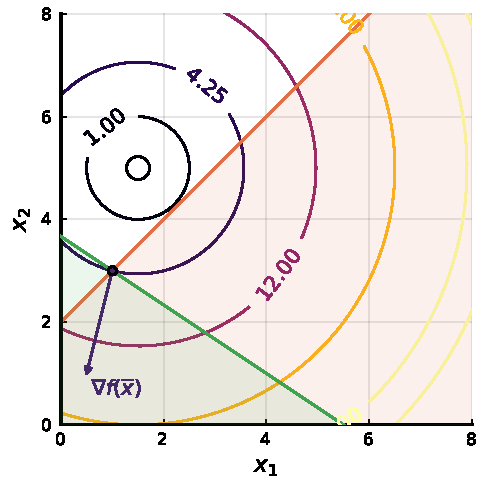
\includegraphics{part_2/chapter_4/figures/ex1.pdf}
	\caption{Example 1}	\label{fig:ex_1}
\end{figure}

The arrow shows the gradient $\nabla f(\overline{x})$ at $\overline{x} = (1,3)$. Notice that this point is special since at that point, no vector $x - \overline{x}$ can be found forming an angle greater than 90$^\circ$ with $\nabla f(\overline{x})$, that is $\nabla f(\overline{x})^\top(x - \overline{x}) \geq 0$ for any $x \in S$, which means that $\overline{x}$ is optimal. Since the problem is convex, that is in fact the global optimum for this problem.

Figure \ref{fig:ex_2} shows a similar situation, but now with one of the constraints being nonlinear. Notice that of the two points highlighted ((1,2) in orange and (2,1) in purple), the optimality condition only holds for (2,1). For example, for $x = (2,1)$ and $\overline{x} = (1,2)$ the vector $x - \overline{x}$ forms a angle greater than 90$^\circ$ with the gradient of $f$ at $\overline{x}$, $\nabla f(\overline{x})$, and thus the condition $\nabla f(\overline{x})^(x - \overline{x}) \geq 0$ does not hold for all $S$. The condition does hold for $\overline{x} = (2,1)$, as can be seen in Figure \ref{fig:ex_2}.  

\begin{figure}[H]
	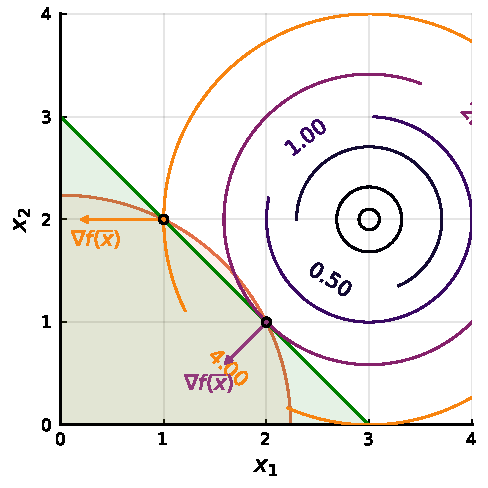
\includegraphics{part_2/chapter_4/figures/ex2.pdf}
	\caption{Example 2}	\label{fig:ex_2}
\end{figure}

A geometrical interpretation of the optimality condition $\xi^\top(x - \overline{x}) \geq 0$ is as follows. If there exists a subgradient $\xi$ (or a gradient $\nabla f(\overline{x})$ if $f$ is differentiable) that serves as a separating hyperplane between the level curve of $f$ at $\overline{x}$ and the feasible region $S$, then there can be no feasible point further into the lower level set defined by that level curve. Ultimately, this means that there is no feasible point with smaller objective function value to be found. This is why the separation theorem from Lecture 2 plays an important role here, since it can be used to state that the feasible options have been exhausted in terms of potential directions of decrease of objective function value.  

\subsection{Optimality conditions for unconstrained problems}

We have developed most of the concepts required to state optimality conditions for unconstrained optimisation problems, as presented in Corollaries \ref{cor:opt_conditions_open} and \ref{cor:opt_conditions_diff}. We now take an alternative route in which we do not take into account the feasibility set, but only the differentiability of $f$. This will be useful as it will allow us to momentarily depart from the assumption of convexity, which was used to state Theorem \ref{thm:opt_conditions}. 

\subsubsection{First-order optimality conditions}

Let us start defining what it means to be a \emph{descent direction}.

\begin{theorem}[descent direction]\label{thm:descent_dir}
Suppose $f: \reals^n \mapsto \reals$ is differentiable at $\overline{x}$. If there is $d$ such that $\nabla f(\overline{x})^\top d < 0$, there exists $\delta > 0$ such that $f(\overline{x} + \lambda d) < f(\overline{x})$ for each $\lambda \in (0, \delta)$, so that $d$ is a descent direction of $f$ at $\overline{x}$.
\end{theorem}
%
\begin{proof}
By differentiability of $f$ at $\overline{x}$, we have that 
\begin{align*}
\frac{f(\overline{x} + \lambda d)-f(\overline{x})}{\lambda} = \nabla f(\overline{x})^\top d + ||d||\alpha(\overline{x};\lambda d).
\end{align*}
Since $\nabla f(\overline{x})^\top d < 0$ and $\alpha(\overline{x};\lambda d) \rightarrow 0$ when $\lambda \rightarrow 0$ for some $\lambda \in (0, \delta)$, we must have $f(\overline{x} + \lambda d)-f(\overline{x}) < 0$.
\end{proof}

The proof uses the first-order expansion around $\overline{x}$ to show that, $f$ being differentiable, the condition $\nabla f(\overline{x})^\top d < 0$ implies that $ f(\overline{x} + \lambda d) < f(\overline{x})$, or put in words, that a step in the direction $d$ decreases the objective function value.

We can derive the first-order optimality condition in Corollary \ref{cor:opt_conditions_diff} as a consequence from Theorem \ref{thm:descent_dir}. Notice, however, that since convexity is not assumed, all we can say is that this condition is necessary (but not sufficient) for local optimality.

\begin{corollary}[first-order necessary condition]\label{thm:suff_first_order_cond}
Suppose $f: \reals^n \rightarrow \reals$ is differentiable at $\overline{x}$. If $\overline{x}$ is a local minimum, then $\nabla f(\overline{x}) = 0$.
\end{corollary}
%
\begin{proof}
By contradiction, suppose that $\nabla f(\overline{x}) \neq 0$. Letting $d = -\nabla f(\overline{x})$, we have that  $\nabla f(\overline{x})^\top d = -||\nabla f(\overline{x})||^2 < 0$. By Theorem \ref{thm:descent_dir}, there exists a $\delta > 0$ such that $f(\overline{x} + \lambda d) < f(\overline{x})$ for all $\lambda \in (0, \delta)$, thus contradicting the local optimality of $\overline{x}$. 
\end{proof}

Notice that Corollary \ref{thm:suff_first_order_cond} only holds in one direction. The proof uses contradiction once again, where we assume local optimality of $\overline{x}$ and show that having $\nabla f(\overline{x}) \neq 0$ contradicts the local optimality of $\overline{x}$, our initial assumption. To do that, we simply show that having any descent direction $d$ (we use $-\nabla f(\overline{x})$ since in this setting it is guaranteed to exist as $\nabla f(\overline{x}) \neq 0$) would mean that small step $\lambda$ can reduce the objective function value, contradicting the local optimality of $\overline{x}$. 


\subsubsection{Second-order optimality conditions}

We now derive necessary conditions for local optimality of $\overline{x}$ based on second-order differentiability. As we will see, it requires that the Hessian $H(\overline{x})$ of $f(x)$ at $\overline{x}$ is positive semidefinite.
%
\begin{theorem}[second-order necessary condition]\label{thm:second_order}
Suppose $f: \reals^n \rightarrow \reals$ is twice differentiable at $\overline{x}$. If $\overline{x}$ is a local minimum, then $H(\overline{x})$ is positive semidefinite.
\end{theorem}
%
\begin{proof}
Take an arbitrary direction $d$. As $f$ is twice differentiable, we have:
%
\begin{align*}
f(\overline{x} + \lambda d) = f(\overline{x}) + \lambda \nabla f(\overline{x})^\top d + \frac{1}{2}\lambda^ 2d^\top H(\overline{x}) d + \lambda^2||d||^2\alpha(\overline{x}; \lambda d)
\end{align*}
%
since $\overline{x}$ is a local minimum, Corollary \ref{thm:suff_first_order_cond} implies that $\nabla f(\overline{x})=0$ and $f(\overline{x} + \lambda d) \geq f(\overline{x})$. 

Rearranging terms and dividing by $\lambda^2 > 0$ we obtain
$$\frac{f(\overline{x} + \lambda d)-f(\overline{x})}{\lambda^2} =  \frac{1}{2}d^\top H(\overline{x}) d+ ||d||^2\alpha(\overline{x};\lambda d).
$$
Since $\alpha(\overline{x};\lambda d) \rightarrow 0$ as $\lambda \rightarrow 0$, we have that $d^\top H(\overline{x}) d \geq 0$.
\end{proof}

The second-order conditions can be used to attest local optimality of $\overline{x}$. In the case where $H(\overline{x})$ is positive definite, then this second order condition becomes \emph{sufficient} for local optimality, since it implies that the function is 'locally convex' for a small enough neighbourhood $N_\epsilon(\overline{x})$.

In case $f$ is convex, then the first-order condition $\nabla f(x) = 0$ becomes also sufficient for attesting the global optimality of $\overline{x}$. Recall that $f$ is convex if and only if $H(x)$ is positive semidefinite for all $x \in \reals^n$, meaning that in this case the second-order necessary conditions are also satisfied at $\overline{x}$.
%
\begin{theorem}
Let $f: \reals^n \mapsto \reals$ be convex. Then $\overline{x}$ is a global minimum if and only if $\nabla f(\overline{x}) = 0$.
\end{theorem}
%
\begin{proof}
From Corollary \ref{thm:suff_first_order_cond}, if $\overline{x}$ is a global minimum, then $\nabla f(\overline{x}) = 0$. Now, since $f$ is convex, we have that
%
\begin{align*}
f(x) \geq f(\overline{x}) + \nabla f(\overline{x})^\top (x - \overline{x})
\end{align*}
%
Notice that $\nabla f(\overline{x}) = 0$ implies that $\nabla f(\overline{x})^\top (x - \overline{x}) = 0$ for each $x \in \reals^n$, thus implying that $f(\overline{x}) \leq f(x)$ for all $x \in \reals^n$.
\end{proof}
